This chapter describes the methods and materials used throughout the study to address the research questions of the study (Section \todo{add section number}).
Details of the modelling set-up, including initial and boundary conditions are included in this chapter.

\section{Air Quality Modelling} \label{s:modelling}

Photochemical models are used to predict future air quality scenarios.
A large array of these models are used depending on the study focus, for example, global photochemical models can predict air quality on a global scale and include the relevant chemical and dynamical processes whereas an urban model focuses on a particular urban area and includes the relevant processes (such as topography, local emission source) to the area being studie.
Despite differing scopes between models, there are a number of common inputs including emissions of chemical species into the model, transport of the species, atmospheric physical and chemical transformation and numerical solutions to the applicable differential equations.

Models are usually defined as either Eulerian or Lagrangian, with Eulerian models constituting most of the models used in the air quality modelling community \citep{Russell:2000}.
Eulerian models describe the atmosphere by fixed computational cells where species enter in and out of the cell walls and the concentrations of the species within each cell are calculated as a function of time. 
Whilst Lagrangian models simulate changes of selected air parcels during advection through the atmosphere, hence there is no mass exchange between the surroundings and the air parcel (besides the emissions) and the model calculates concentrations at different locations at different times \citep{Seinfeld:2006}. 

Photochemical models also have different dimensions, ranging from zero-dimensional (box model) to three-dimensional models where the simplicity and computing power increase with the dimension of the model.
3-D models calculate atmospheric concentrations as a function of latitude, longitude, altitude and time. 
While 2-D models assume that concentration is a function of latitude and altitude (but not longitude) and time.
Column models (or 1-D models) use concentrations that are a function of time and height.
Box models are the simplest type of a model and have uniform atmospheric concentrations that are only a function of time \citep{Seinfeld:2006}.

Box models lack physical realism and essentially focus on processes relevant to a point in the atmosphere.
Despite the lack of realism, box models are extremely useful for studying the detailed processes that influence air quality.
Examples of modelling studies that have used box models include \citet{Bin:2007}, \citet{Li:2014b} and \citet{Noelscher:2014}.

All photochemical models numerically solve the chemical species conservation equation which describes the processes affecting the concentration of the different species:
\begin{equation} \label{e:conc}
    \begin{split}
        \frac{\partial c_i}{\partial t} \hspace{2mm} + \hspace{2mm} \nabla \cdot \bar{U}c_i \hspace{2mm} = \hspace{2mm} \nabla \rho D \nabla(c_i/\rho) \hspace{2mm} + \hspace{2mm} R_i(c_1, c_2, \dots, c_n, T, t) \\ + \hspace{2mm} S_i(\bar{x}, t), \hspace{5mm} i = 1, 2, \dots, n.
    \end{split}
\end{equation}
In Eq.~\eqref{e:conc}, $c_i$ is the concentration (in mass or volume) of species $i$, $\bar{U}$ is the wind velocity vector, $D_i$ is the molecular diffusivity of species $i$, $R_i$ is the rate of concentration change of species $i$ through chemical reactions, $S_i(\bar{x}, t)$ is the source or sink of $i$ at location $\bar{x}$, $\rho$ is the air density and $n$ is the number of predicted species.
$R$ may also be a function of meteorological parameters such as temperature $T$ and $S$ includes emission and deposition processes affecting $i$ \citep{Russell:2000}.
\todo{re-word this as too similar to citation}

The dimension and type of the model determine the set of differential equations that will be solved at each time step of the model run. 
Numerical methods to determine the concentration of species $i$ in Eq.~\eqref{e:conc} vary between models, examples include Runge-Kutta \citep{Sandu:1997b}, Finite Element \citep{Russell:2000} or Rosenbrock methods \citep{Sandu:1997a}.

Initial and boundary conditions are required to numerically solve the system of differential equations.
Boundary conditions are typically the most difficult input to set accurately as this requires knowledge of the investigated species concentrations and transport at the boundary edges (if applicable) of the model grid.  
Setting the initial conditions involves fixing the starting concentrations of the species being studied, these conditions are dependent on the area being studied and whether it is an urban or rural area, amongst other considerations. 

\subsection{Model Description and Setup}
In order to assess the detailed processes producing tropospheric ozone within general air quality modelling, we used a box model to focus on the gas-phase chemistry affecting tropospheric ozone.
All simulations in this study were performed using the MECCA (Module Efficiently Calculating the Chemistry of the Atmosphere) box model developed by \citet{Sander:2005} that was adapted to include MCM~v3.1 chemistry as described in \citet{Butler:2011}.
The MECCA box model has been used for numerous detailed process studies of atmospheric gas-phase chemistry including \citet{Kubistin:2010}, \citet{Xie:2008} and \citet{Lourens:2012}.

MECCA is written using the FORTRAN programming language and runs on UNIX/Linux platforms.
The setup of MECCA that we used uses the KPP (Kinetic Pre-Processor) \citep{Damian:2002} to efficiently setup up the system of differential equations (Eq.~\eqref{e:conc}).
KPP processes the specified chemistry scheme in the chemical mechanism and generates Fortran code that is then compilied by MECCA.
KPP also has numerous choices for the numerical solver used to numerically determine the concentrations of all the species described by the chemistry.
We have used a Rosenbrock solver (the ros3 option) throughout the study.

Aside from the chemistry, MECCA also calculates physical parameters at every time step of the simulations.
In our simulations, the pressure, temperature, relative humidity and boundary layer height are held constant at the set values of Table~\ref{t:model_setup}.
The specific changes to these parameters that were systematically varied to answer the research question related to \todo{add section} are detailed in the relevant publication (Chapter ). \todo{TBC about this}

\begin{table}
    \begin{center}
        \caption{General settings used for MECCA box model in this study}
        \begin{tabular}{ll}
            \hline \hline
            \textbf{Model Parameter} & \textbf{Setting} \\
            \hline \hline
            Pressure & $1013$ hPa \\
            Temperature & $293$ K \\
            Relative Humidity & $81$ \% \\
            Boundary Layer Height & $1000$ m \\
            Latitude & $34\degree$ N \\
            Starting Date and Time & 27th March 06:00 \\
            Model Time Step & $20$ mins \\
            Model Run Time & $7$ days \\
            \hline \hline
        \end{tabular}
        \label{t:model_setup}
    \end{center}
\end{table}

Photolysis rates in this study are calculated by using a paramaterisation that calculates the photolysis rate as a function of the solar zenith angle.
This paramaterisation requires the degree of latitude for the study to be a defined variable in MECCA, we have chosen the $34\degree$ N latitude which is roughly that of the city of Los Angeles.
The simulations start at the spring equinox (27th March) at 6am and allowed to run for seven diurnal cycles.

In our setup of MECCA, all fluxes into and out of the box are handled by KPP.
The chemical mechanism file, processed by KPP, includes specific pseudo-unimolecular reactions specifying the emissions and dry deposition of chemical species along with the relevant rate.
The chemical species that are emitted into the model and the emission rates are read into the model using a namelist file.
Namelist files are also used to specify the initial conditions of chemical species and the mixing ratios of those chemical species that are fixed throughout the model.
In all simulations, methane (\ce{CH4}) was fixed to 1.75 ppmv while carbon monoxide (CO) and \ce{O3} are initialised at 200 ppbv and 40 ppbv and then allowed to evolve freely.

\section{Chemical Mechanisms}
Models use chemical mechanisms to implement the atmospheric chemistry at each time step during a model run. 
The mechanism includes rate coefficients, reaction pathways with the corresponding branching ratios, photolysis rates and reaction products, amongst other parameters. 
This part of a model consumes a great deal of the computing resources, hence, when using a three-dimensional model the mechanism will include less chemical detail compared to a study incorporating a box-model. 
To achieve this, mechanisms used primarily in three-dimensional models will aggregate compounds, include more assumptions about how reactions proceed and how the degradation products are treated when compared to mechanisms used in box-modelling studies.

The Master Chemical Mechanism (MCM) in \citep{Saunders:2003, Jenkin:2003} is a near-explicit mechanism that is used for box modelling studies. 
Regional and global mechanisms include the Regional Atmospheric Chemistry Mechanism (RACM), the Carbon Bond Mechanism (CB-05 in \citep{Yarwood:2005}), the National Center for Atmospheric Research (NCAR) master mechanism (\citep{Madronich:1989}) and the Statewide Air Pollution Research Center (SAPRC), although many mechanisms include reduced mechanisms that are applicable to different model dimensions. 

\subsection{Self-Generating Mechanisms}
The self-generating mechanism is the type of chemical mechanism that reflects the details of the atmospheric chemistry summarised in Section \ref{s:atmo_chem} the most and is also called an explicit mechanism. 
This requires thousands of reactions as the degradation of minor products is often more complex than that of the parent VOC. 
It also represents a compact method of obtaining a detailed mechanism that describes tropospheric chemistry.

\citep{Aumont:2005} outlines a way of including all reaction pathways that does not imply manually writing all the reactions with their respective parameters, as is the case for other mechanisms. 
This would also include the possibilty of heterogeneous chemistry and aerosol formation being accouted for in the mechanism, these are aspects of atmospheric chemistry that are not treated in great detail in chemical mechanisms used for gas-phase calculations.

The approach in \citep{Aumont:2005} is to write a so-called `generator' program that analyses the chemical structure of the VOC being studied to determine the reactive sites which then give the reaction pathways. 
The generator then accesses another file which includes the available reaction parameters and the reaction products. 
Structure activity relationships (SARs) are used when no reaction parameters are available. 
A file is then created that contains the final reaction, it includes the reactants, products and rate coefficients amongst other information. 
This process is then repeated for the products until all the oxidation reactions have been completed.

There are a number of advantages of this type of mechanism over mechanisms that are manually written up reaction by reaction. 
Firstly, a self-generating mechanism is faster to write since there are less reactions that need to be written due to the use of a generator program. 
This also implies increased accuracy (less manually written reactions means less typographical errors) and also maintenance is much easier as far less code needs to be updated. 
Currently, this type of mechanism has not been used in relation to ozone production potential calculations. 

\subsection{Master Chemical Mechanism}
The Master Chemical Mechanism (MCM) v3.2 is a near-explicit mechanism describing the chemical degradation of 107 non-aromatic VOCs in \citep{Saunders:2003} and 18 aromatic VOCs in \citep{Jenkin:2003}. 
In total the MCM v3.2 has 12,691 reactions including 4351 organic compounds and 46 associated inorganic compounds. 
The MCM includes alkanes, alkenes, dienes, monoterpenes, aromatics, aldehydes and ketones amongst others, the complete list is found online (\url{http://mcm.leeds.ac.uk/MCM/}). 
The VOCs were chosen in accordance with the UK National Atmospheric Emissions Inventory and include those that make up about 70\% of the mass emissions of unique species achieved.

Each primary VOC and each degradation product, is individually degraded until it is broken down to \ce{CO2}, CO or an organic product (or radical) already found in the MCM \citep{Jenkin:1997}. 
The main assumptions made to reduce the number of reactions and compounds in the MCM are given below and are taken from \citep{Jenkin:1997}.
\begin{enumerate}
    \item The number of product channels resulting from reaction with the OH radical is limited by disregarding those pathways of low probability.
    \item Many permutation (i.e. self and cross) reactions of organic peroxy radicals are represented by a single parameterised reaction. This is particularly required as inclusion of all peroxy radical reactions would involve about 400,000 reactions.
    \item The degradation chemistry is simplified, especially for those ``side" products deemed to be minor.
\end{enumerate}
Figure \ref{f:MCM_scheme} shows the reaction pathways represented in the MCM of a primary VOC, these shall be summarised below.
First the schemes used for the degradation reactions of non-aromatic VOCs in \citep{Saunders:2003} shall be discussed. 
As mentioned above, the main reaction pathway for VOC degradation is by OH radical reaction and hence this is included for the vast majority of VOCs considered. 
Reaction with \ce{O3} is deemed to only be important for alkenes, dienes, monoterpenes and some unsaturated oxygenated products. 
Reaction with the \ce{NO3} radical is mainly important during the night-time and for alkenes, dienes, aldehydes and ethers.  

For all reactions in the MCM, rate coefficients are taken from literature, where available, if not then they are estimated using methods also described in literature (for example, via SAR and group reactivity (GR) methods). 
The branching ratios of all reactions are also taken or estimated from literature. 
The reactions with \ce{O3} and the \ce{NO3} radical are also included if the parent VOC has a rate of removal that is more than 1\% of its removal rate with the OH radical and its lifetime with respect to reaction with \ce{O3} (or \ce{NO3}, accordingly) is less than $10^7$ seconds.
\begin{figure}
    \begin{center}
        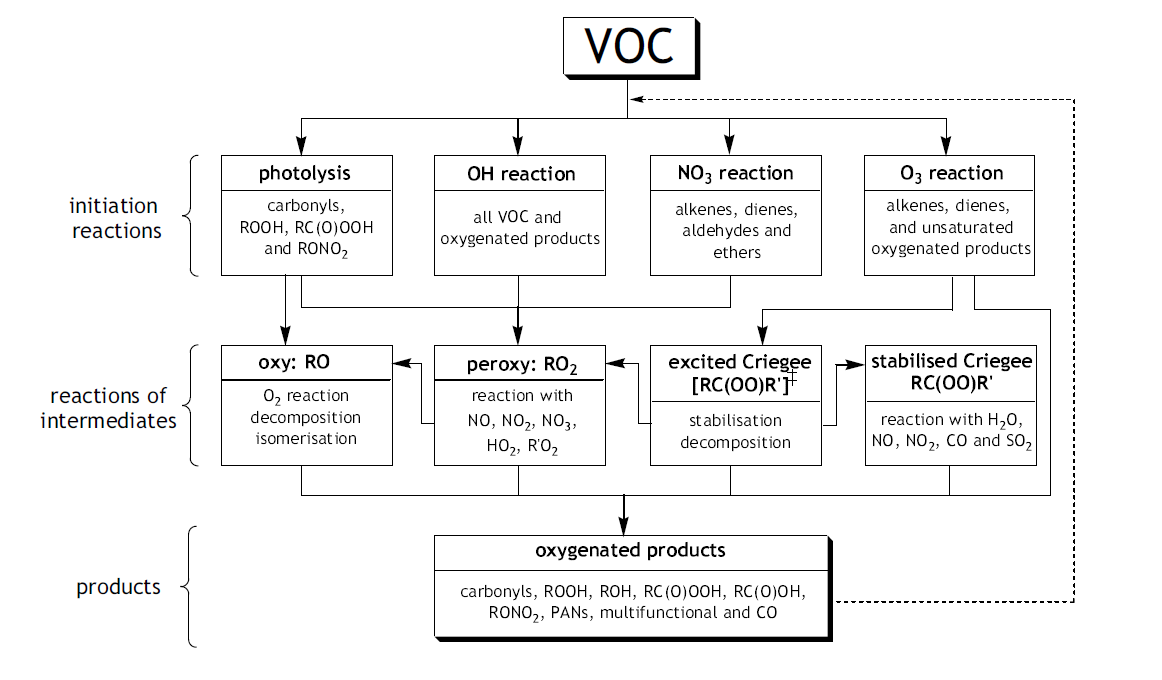
\includegraphics[width=13cm]{MCM_scheme.png}
        \caption{Flowchart of the major reactions, reactions of intermediates and products considered in the MCM. Taken from \citep{Saunders:2003}}
        \label{f:MCM_scheme}
    \end{center}
\end{figure}

Photolysis is included for those compounds that absorb at wavelengths less than 290 nm. 
The photolysis parameters are given for those  compounds for which absorption cross-sections and quantum yield data is known and they are also determined as a function of the solar zenith angle. 

The degradation products are also treated in detail, these first generation products are also degraded further as part of the MCM. 
Those products that have significant tropospheric concentrations are already treated in the MCM. 
To simplify this part of the mechanism, the products are limited to their reaction pathways with the OH radical. 
Those products which are deemed as minor are also greatly simplified whilst retaining product lifetimes and maintaining the carbon and nitrogen balance. 
However, many of these reactions are unbalanced in their \ce{O2} or \ce{H2O} output \citep{Jenkin:1997}. 
The kinetic data, where available, is taken from literature however mainly SAR estimations are used due to the lack of data.

In \citep{Jenkin:2003} the treatment of the aromatic VOCs included in the MCM v3.2 is described, this is summarised below. 
Where possible the treatment follows that of non-aromatic VOCs as outlined above and in \citep{Saunders:2003}. 
However this is not possible for many reactions due to the intricacies of aromatic VOC chemistry and the fact that there is a lack of knowledge of the detailed degradation schemes. 
Also, similar simplifications are again present to reduce the complexity of the mechanism, this is particularly true for the \ce{C6 - C11} aromatic compounds.

Reaction with the OH radical is the main reaction pathway of aromatic compounds, the relevant rate coefficients are taken from literature, where available, or estimated depending on the functional group \citep{Jenkin:2003}. 
The reaction pathways are known to proceed by H-atom abstraction or by addition to the aromatic ring. 
The branching ratios are taken from literature or applied from the analogous molecule for which there is information. 
H-atom abstraction is typically deemed to be a minor pathway, at this point the simplification applied is that only one pathway during the initial OH radical attack is chosen. 
Literature provides the data at which point in the aromatic ring the addition reaction occurs and also the following reaction with \ce{O2}. 
Some specific cases are treated separately according to the relevant literature \citep{Jenkin:2003}.

The previous conditions outlined above for reaction with \ce{O3} and with the \ce{NO3} radical are also applied to aromatics VOCs. 
Again, all rate coefficients and branching ratios are either taken or estimated from the available data and the reaction pathways also proceed as described in literature. 
Photolysis is only considered for some aromatic VOCs based on the conditions described above. 
For those cases in which data are not available, the photolysis rates are taken by extension of the data available \citep{Jenkin:2003}. 
Hence, all reactions proceed as described in literature with estimations used for those cases lacking data.

The degradation products are also further degraded in the MCM, these are split into two general groups - those still containing an aromatic ring and those formed after ring-opening. 
The latter are then treated as non-aromatic compounds as described above in \citep{Saunders:2003}. 
The former group is then further divided into four categories depending on the resulting product and these are then degraded according to \citep{Jenkin:2003}.

\subsection{Regional Atmospheric Chemistry Mechanism}
Another chemical mechanism is the Regional Atmospheric Chemistry Mechanism (RACM), described in \citep{Stockwell:1997} and described below. 
This is a complete revision of the Regional Acid Deposition (RADM2) mechanism and is applicable to regional modelling and capable of simulating the gas phase tropospheric chemistry over remote and heavily polluted urban regions, including at the Earth's surface and in the upper troposphere. 
The RACM includes 17 inorganic, four inorganic intermediates and 32 organic species, four of which are of biogenic origin that altogether entail about 237 reactions. 
The inorganic reactions are practically fully described with the relevant rate coefficients, quantum yields and photolysis coefficients taken from literature.

In order to reduce computational resources for the mechanistic part of a regional model, the organic compounds are grouped into 16 anthropogenic and three biogenic model species. 
This grouping is based upon emission rates, functional group similarity and OH radical reactivity. 
Obtaining the final model species was done in two steps, first the hundreds of anthropogenic VOCs were grouped into 32 emission categories and then these were aggregated into the final 16 model species. 
Another aspect of reducing computational requirements was achieved by reducing the number of reaction pathways by only taking one reaction pathway from those available and also not treating all the organic intermediates explicitly.

The reaction rate coefficients of the model species are obtained by a weighted mean of all the rate coefficients of the organic species aggregated into the model species, this is done to account for the difference in reactivities between the model and chemical species. 
The individual rate coefficients are taken from literature or estimated by means of a SAR. 
Some organic compounds (for example, methane and ethene) are explicitly treated, if not then the compounds are represented by a model species. 
For example, excluding ethene, anthropogenic alkenes with their double bond at the end of the molecule are included as the model species as OLT whilst anthropogenic alkenes with their double bond not at the end of the molecule are represented by OLI \citep{Stockwell:1997}.

The different functional groups in a model species give rise to different reaction products, hence other model species are introduced with the relevant product yield fractions, as illustrated in the below reactions.
\begin{reactionlist}
    \reactionitem{OLT + OH}{OLTP}{new}{r:OLT+OH}
    \reactionitem{OLI + OH}{OLIP}{new}{r:OLI+OH}
\end{reactionlist}
These product species are calculated as a weighted mean of the product yields of all the chemical species represented by the model species, where the individual yields are taken from literature. 

The branching ratios of certain reactions are also parameterised, for example the slow-reacting aromatic species, represented by the model species TOL, are assumed to react with the OH radical by addition to the aromatic ring with a 0.1 fraction of the reactions proceeding by H-atom abstraction.
\begin{reactionlist}
    \reactionitem{TOL + OH}{0.90 ADDT + 0.10 \ce{XO2} + 0.10 \ce{HO2}}{new}{r:TOL+OH}
\end{reactionlist}
Furthermore, the branching ratios of the reactions of the aromatic-OH adduct (ADDT) are determined by simulating the environmental chamber data and this calculation is dependent on the secondary products formed from the reactions of unsaturated dicarbonyls. 
This is a source of uncertainity in the mechanism and since these three pathways after the \ce{O3} production rate, obtaining the correct branching ratio is of importance \citep{Stockwell:1997}.

The model species \ce{XO2} is used to represent peroxy radicals where the appropriate \ce{XO2} radical is dependent on the rate coefficient of the generating reaction. 
Also, the product yields are once again obtained via a weighted mean of the product yields of the individual species. 
To paramaterise the vast amount of reactions, very fast reactions are ignored and reactions with \ce{O3} are estimated due to the lack of experimental data. 

\citep{Kirchner:1996} details the treatment of organic peroxy radicals. 
The organic-peroxy radical-organic peroxy radical reactions are represented by reactions of the organic-peroxy radical with the two most important peroxy radicals (\ce{CH3O2} and \ce{CH3C(O)O2}) and all other reactions with organic-peroxy radicals are ignored. 
The reaction rate coefficients of organic-peroxy radical self and cross reactions were estimated using the method described in \citep{Kirchner:1996}. 
Experimental data is used for the rate coefficients of alkyl peroxy radicals reaction with NO. 

\section{Comparison of Chemical Mechanisms}
Given the different chemical mechanisms and their differing approaches towards simplifying the complexities of atmospheric chemistry, there have been many comparative studies to determine the differences between calculation results obtained when performing the same modelling study but altering the mechanism. 
In \citep{Dunker:1984} four mechanisms that were used in atmospheric modelling studies were compared by means of atmospheric simulations of box, trajectory and grid modelling studies and also against chamber study results. 
The comparison parameters were plotted \ce{O3}, \ce{NO2} and PAN isopleths as well as the time span required for the maximum one hour average \ce{O3}, \ce{NO2} and PAN concentrations to be reached. 
The largest differences between the mechanisms were found during the box model study whereas the other simulations correlated well. 
It is also highlighted that differences in chemistry can be masked by the effects of the meteorology and other parameters not included in a box model.

A study of the chemical mechanisms used mainly for European regional studies are compared in \citep{Gross:2003}. 
Here, a box model study with the three different mechanisms is used to generate the concentrations of \ce{O3}, NO, \ce{NO2}, \ce{OH} radical, \ce{HO2} radical and organic peroxy radicals \ce{RO2}. 
\ce{O3} isopleth plots are also generated by performing the study over a range of \ce{NO_x} and VOC concentrations. 
A common set of photolysis coefficients were used so that the results would mirror only differences in the chemistry, the study also accounted for both urban and rural conditions in separate model runs.

The results show that the greatest differences between these mechanisms are in the \ce{O3}, \ce{NO2} and \ce{RO2} radical concentrations. 
The differences in the \ce{O3} concentrations are linked to the discrepancies between the \ce{NO2} and \ce{RO2} concentrations as these are reactions that lead to \ce{O3} production or loss. 
This emphasises the importance of the treatment of organic peroxy radicals, which is typically one of the major areas of difference between chemical mechanisms. 
The rural study showed little difference in the comparison parameters whilst the urban study showed larger differences. 
This can be attributed to the complexity of the organic chemistry prevalent in urban areas. 
\citep{Gross:2003} recommends that many different urban scenarios be considered and that \ce{O3} isopleth plots giving the \ce{O3} concentration over a range of \ce{NO_x} and VOC values should be used for such mechanism comparison studies. 

\citep{Emmerson:2009} compares the gas-phase chemical mechanisms used in global models. 
Since the MCM contains more chemical details than the reduced schemes used in global models it is used as a reference to which these are compared. 
The comparison is performed by box model runs simulating a large number of scenarios that are characteristic of global situations - industrial, clean, cold and dry, hot and wet, biogenic and non-biogenic conditions. 
Moreover, a particular recorded event (where the data are taken from the summer 2003 TORCH campaign) is also simulated with all the models to determine how close the simulation results are to the actual recorded concentrations. 

The simulations were ran without heterogenous chemistry and all set to begin at midnight in order to investigate the effect of night-time chemistry, which would be affected most by not including heterogenous chemistry. 
The length of each simulation is five days as a compromise between very long and very short run times which can affect the chemistry in different ways. 
Long model runs would imply significant ageing of the air masses that would drive the chemistry and very short model runs would not test the chemistry pertaining to the degradation products at all, hence a compromise needs to be found. 
Separate model runs were also performed to determine differences in the inorganic chemistry, full chemistry and night-time chemistry.

The resulting concentrations of specific compounds were plotted and compared to verify where mechanistic differences arise. 
The little difference between inorganic chemistry regimes can be attributed to the differences between kinetic data supplied by IUPAC and JPL, whilst there are more differences between the full chemistry and night-time chemistry. 
The greatest differences in the organic chemistry is when biogenic compounds, such as isoprene, are considered and are present in larger concentrations. 
For the specific pollution event that was modelled, the greatest differences arise for the night-time chemistry and \ce{O3} concentrations.

Reactivity scales have also been used as comparison tool for chemical mechanisms, this was proposed as in a single number, they provide a lot chemical kinetic data. 
In \citep{Derwent:2010}, the MCM and SAPRC are compared by calculation of the POCP of 116 organic compounds from the major atmospheric classes within both mechanisms. 
A series of photochemical trajectory model runs simulating a single day were performed, many parameters other than the mechanisms were adjusted as incremental reactivities are not solely geophysical measures but rely on many other parameters.

The MCM and the SAPRC were chosen for this study as they are near-explicit mechanisms with the main difference being in how they treat the first generation products - the MCM continues in an explicit manner while the SAPRC uses aggregation techniques. 
In general, the POCP values correlate very well between the two mechanisms, with a small number of exceptions. 
These can be attributed to the lack of detailed understanding of the degradation reactions of these compounds. 
The good correlation of reactivities of the aromatic compounds merely indicates that both mechanisms treat aromatic compounds similarly rather than having a detailed knowledge of these degradation schemes.

A detailed look at the chemistry affecting different mechanisms used in air quality modelling is described in \citep{Stockwell:2012}, where a box modelling study is undertaken with near-explicit and aggregated chemical mechanisms. 
The model system used is the same as that used in \citep{Seefeld:1999} with only gas-phase chemistry and constant meteorological conditions.  
Different model runs were also undertaken with different temperatures in order to determine the temperature dependency of model results. 

The study highlights that the temperature dependence of gas phase reactions is uncertain for both organic and inorganic compounds. 
Also, night-time chemistry is a major source of uncertainty. 
Other knowledge gaps include the rate coefficients of the reactions of organic peroxy radicals as well as the products resulting from these reactions, the detailed degradation of both aromatic and biogenic compounds.  
